% !TEX encoding = UTF-8 Unicode
\documentclass[a4paper,12pt]{article}
	
	% В этом документе преамбула
	
	%%% Работа с русским языком
	\usepackage{cmap}					% поиск в PDF
	\usepackage{mathtext} 				% русские буквы в формулах
	\usepackage[T2A]{fontenc}			% кодировка
	\usepackage[utf8]{inputenc}			% кодировка исходного текста
	\usepackage[english]{babel}	% локализация и переносы
	\usepackage{indentfirst}
	\frenchspacing
	
	\renewcommand{\epsilon}{\ensuremath{\varepsilon}}
	\renewcommand{\phi}{\ensuremath{\varphi}}
	\renewcommand{\kappa}{\ensuremath{\varkappa}}
	\renewcommand{\le}{\ensuremath{\leqslant}}
	\renewcommand{\leq}{\ensuremath{\leqslant}}
	\renewcommand{\ge}{\ensuremath{\geqslant}}
	\renewcommand{\geq}{\ensuremath{\geqslant}}
	\renewcommand{\emptyset}{\varnothing}
	
	%%% Дополнительная работа с математикой
	\usepackage{amsmath,amsfonts,amssymb,amsthm,mathtools} % AMS
	\usepackage{icomma} % "Умная" запятая: $0,2$ --- число, $0, 2$ --- перечисление
	
	%% Номера формул
	%\mathtoolsset{showonlyrefs=true} % Показывать номера только у тех формул, на которые есть \eqref{} в тексте.
	%\usepackage{leqno} % Нумереация формул слева
	
	%% Свои команды
	\DeclareMathOperator{\sgn}{\mathop{sgn}}
	
	%% Перенос знаков в формулах (по Львовскому)
	\newcommand*{\hm}[1]{#1\nobreak\discretionary{}
		{\hbox{$\mathsurround=0pt #1$}}{}}
	
	%%% Работа с картинками
	\usepackage{graphicx}  % Для вставки рисунков
	\setlength\fboxsep{3pt} % Отступ рамки \fbox{} от рисунка
	\setlength\fboxrule{1pt} % Толщина линий рамки \fbox{}
	\usepackage{wrapfig} % Обтекание рисунков текстом
	
	%%% Работа с таблицами
	\usepackage{array,tabularx,tabulary,booktabs} % Дополнительная работа с таблицами
	\usepackage{longtable}  % Длинные таблицы
	\usepackage{multirow} % Слияние строк в таблице
	
	%%% Теоремы
	\theoremstyle{plain} % Это стиль по умолчанию, его можно не переопределять.
	\newtheorem{theorem}{Theorem}
	\newenvironment{Proof} % имя окружения
	{\par\noindent{\bf Proof.}} % команды для \begin
	{\hfill$\scriptstyle\blacksquare$} % команды для \end
	
	\newtheorem{proposition}[theorem]{Утверждение}
	
	\theoremstyle{definition} % "Определение"
	\newtheorem{corollary}{Следствие}[theorem]
	\newtheorem{problem}{Задача}[section]
	
	\theoremstyle{remark} % "Примечание"
	\newtheorem*{nonum}{Решение}
	
	%%% Программирование
	\usepackage{etoolbox} % логические операторы
	
	%%% Страница
	\usepackage{extsizes} % Возможность сделать 14-й шрифт
	\usepackage{geometry} % Простой способ задавать поля
	\geometry{top=25mm}
	\geometry{bottom=35mm}
	\geometry{left=35mm}
	\geometry{right=20mm}
	%
	%\usepackage{fancyhdr} % Колонтитулы
	% 	\pagestyle{fancy}
	%\renewcommand{\headrulewidth}{0pt}  % Толщина линейки, отчеркивающей верхний колонтитул
	% 	\lfoot{Нижний левый}
	% 	\rfoot{Нижний правый}
	% 	\rhead{Верхний правый}
	% 	\chead{Верхний в центре}
	% 	\lhead{Верхний левый}
	%	\cfoot{Нижний в центре} % По умолчанию здесь номер страницы
	
	\usepackage{setspace} % �?нтерлиньяж
	%\onehalfspacing % �?нтерлиньяж 1.5
	%\doublespacing % �?нтерлиньяж 2
	%\singlespacing % �?нтерлиньяж 1
	
	\usepackage{lastpage} % Узнать, сколько всего страниц в документе.
	
	\usepackage{soul} % Модификаторы начертания
	
	\usepackage{hyperref}
	\usepackage[usenames,dvipsnames,svgnames,table,rgb]{xcolor}
	\hypersetup{				% Гиперссылки
		unicode=true,           % русские буквы в раздела PDF
		pdftitle={Заголовок},   % Заголовок
		pdfauthor={Автор},      % Автор
		pdfsubject={Тема},      % Тема
		pdfcreator={Создатель}, % Создатель
		pdfproducer={Производитель}, % Производитель
		pdfkeywords={keyword1} {key2} {key3}, % Ключевые слова
		colorlinks=true,       	% false: ссылки в рамках; true: цветные ссылки
		linkcolor=red,          % внутренние ссылки
		citecolor=black,        % на библиографию
		filecolor=magenta,      % на файлы
		urlcolor=blue           % на URL
	}
	
	\usepackage{csquotes} % Еще инструменты для ссылок
	
	%\usepackage[style=authoryear,maxcitenames=2,backend=biber,sorting=nty]{biblatex}
	
	\usepackage{multicol} % Несколько колонок
	
	\usepackage{tikz} % Работа с графикой
	\usepackage{pgfplots}
	\usepackage{pgfplotstable}
	\usepackage{caption}
	\usepackage{subcaption}
	
	\usepackage{algorithm}
	\usepackage[noend]{algcompatible}
	
	\newcommand{\ba}{\mathbf{a}}
	\newcommand{\bb}{\mathbf{b}}
	\newcommand{\bw}{\mathbf{w}}
	\newcommand{\by}{\mathbf{y}}
	\newcommand{\bx}{\mathbf{x}}
	\newcommand{\bz}{\mathbf{z}}
	\newcommand{\cA}{\mathcal{A}}
	\newcommand{\bJ}{\mathbf{J}}
	\newcommand{\bQ}{\mathbf{Q}}
	\newcommand{\bbC}{\mathbb{C}}
	\newcommand{\bbR}{\mathbb{R}}
	\newcommand{\bbY}{\mathbb{Y}}
	\newcommand{\bW}{\mathbf{W}}
	\newcommand{\bH}{\mathbf{H}}
	\newcommand{\bF}{\mathbf{F}}
	\newcommand{\bR}{\mathbf{R}}
	\newcommand{\bX}{\mathbf{X}}
	
	\newcommand{\T}{{\text{\tiny\sffamily\upshape\mdseries T}}}
	\newcommand{\argmin}{\mathop{\arg \min}\limits}
	\newcommand{\argmax}{\mathop{\arg \max}\limits}
	
	
	\begin{document}
		
		\title
	{Quadratic programming optimization for Newton method}
	\date{}
	\maketitle
	\begin{center}
		R.\,V.~Isachenko,
		V.\,V.~Strijov
	\end{center}
	\textbf{Abstract:} 
	To optimize the model parameters the Newton method is widely used. 
	This method is second order optimization procedure that is unstable in real applications. 
	In this paper we propose the procedure to make the optimization process robust. 
	The idea is to select the set of model parameters which have to be optimized in the current step of optimization procedure.
	We show that in the case of nonlinear regression and logistic regression models the parameters selection could be performed by Quadratic Programming Feature Selection algorithm.
	It allows to find the set of independent parameters that are responsible for the residuals.
	We carried out the experiment to show the proposed method {\color{red} TODO}
	
	\bigskip
	\textbf{Keywords}: nonlinear regression, logistic regression, Newton method, quadratic programming feature selection
	
	\section*{Introduction}
	The modern machine learning models have extremely large number of parameters. 
	The error function for such models have ф complex landscape with multiple local minima. 
	The optimization procedure in this case brings to different solutions each time.
	
	The optimization procedure is an iterative process. 
	In each step it updates the current point parameters to get the next approximation.
	There have been developed a lot of first-order optimization algorithms, which use the first derivatives of the error function. 
	The most famous algorithms are SGD, Nesterov momentum~\cite{nesterov1983momentum}, Adagrad~\cite{duchi2011adagrad}, Adam~\cite{kingma2014adam}. 
	These algorithms are widely used for deep neural networks optimization~\cite{goodfellow2016deeplearningbook}. 
	The Newton algorithm is the second-order algorithm which use the second derivatives of the error function. 
	It finds more reasonable updates and converges with much less number of iterations.
	The drawback of the second-order optimization methods huge and ill-conditioned Hessian matrix. 
	The optimization in this case could be computationally expensive and could diverge. 
	To overcome this problem the approximations for the Hessian matrix and regularization are applied~\cite{avriel2003nonlinear,blaschke1997convergence}.
	The paper~\cite{botev2017newtondeeplearning} implements the Newton method to the deep neural networks.
	
	This paper suggests to select the set of model parameters which we optimize in each optimization step.
	We consider nonlinear regression model with squared error function and logistic regression model with cross-entropy error function.
	For nonlinear regression the Newton method and model linearization leads to the Gauss-Newton method. 
	Each step solves the linear regression problem. 
	The authors use the two-layer neural network as the nonlinear model. 
	The Newton method for logistic regression brings to Iteratively Least Squares~(IRLS) algorithm. 
	Here the optimization step is made in the direction given also by the linear regression problem solution.
	
	The paper proposes to apply the Quadratic Programming Feature Selection~(QPFS) algorithm~\cite{katrutsa2017comprehensive,rodriguez2010qpfs} to select the optimal set of model parameters. The QPFS algorithm selects features for the linear regression problem. We have the linear regression problem for both model in each step. The QPFS algorithm tries to maximize the relevances of features and minimize pairwise dependency between features~\cite{ding2005mrmr}. In our case it allows to find independent parameters which impact the model residuals the most.
	
	In the computational experiment we investigate {\color{red} TODO}
	
		
	\section*{Problem Statement}

	The model $f( \bx | \bw), \bw \in \mathbb{R}^p$ predicts the target variable $y \in \bbY$, given the object $\bx \in \bbR^{n}$. The space $\bbY$ equals $\{0, 1\}$ for binary classification problem and $\bbY = \bbR$ for regression problem.
	There are given the design matrix~$\bX = [\bx_1, \dots, \bx_m]^{\T} \in \bbR^{m \times n}$ and the target vector~$\by = [y_1, \dots, y_m]^{\T} \in \bbY^{m}$. 
	The goal is to find the optimal parameters~$\bw^*$.
	The parameters~$\bw$ are fitted by the minimization of the error function:
	\begin{equation}
		\bw^* = \argmin_{\bw \in \bbR^p} S(\bw | \bX, \by, f).
		\label{eq:error_function}
	\end{equation}
	The investigated choices for the error function~$S(\bw | \bX, \by, f)$ are
	squared error for the regression problem: 
		\begin{equation}
			S(\bw | \bX, \by, f) = \frac 12 \| \by - \mathbf{f}(\bX | \bw) \|_2^2 = \frac 12 \sum_{i=1}^m \| y_i - f(\bx_i | \bw)\|^2,
			\label{eq:squared_error}
		\end{equation}
	 and cross-entropy for the binary classification problem: 
		\begin{equation}
			S(\bw | \bX, \by, f) = \sum_{i=1}^m \bigl[y_i \log f (\bx_i | \bw) + (1-y_i) \log (1 - f (\bx_i | \bw))\bigr].
			\label{eq:log_loss}
		\end{equation}
	
	The number of model parameters~$p$ could be extremely huge. 
	The problem~\eqref{eq:error_function} is solved by iterative optimization procedures. 
	To obtain parameters in the step~$k$, the current parameters $\bw^{k-1}$ is updated by the rule
	\begin{equation}
		\bw^k = \bw^{k - 1} + \Delta \bw^{k - 1}.
		\label{eq:update_rule}
	\end{equation}
	This paper suggests to use the Newton optimization procedure to select parameters updates~$\Delta \bw$.

	\section*{Newton method}
	
	The Newton method uses the first order optimization condition for problem~\eqref{eq:error_function} and linearize the gradient of $S(\bw)$
	\[
		\nabla S (\bw + \Delta \bw) = \nabla S(\bw) + \bH \cdot \Delta \bw,
	\]
	\[
		\Delta \bw = - \bH^{-1} \nabla S(\bw).
	\]
	where $\bH = \nabla^2 S(\bw)$ is the Hessian matrix of the error function $S(\bw)$.
	
	The iteration~\eqref{eq:update_rule} of the Newton method is
	\[
		\bw^k = \bw^{k-1} - \bH^{-1} \nabla S(\bw).
	\]
	The Newton method is unstable and computationally hard. Each iteration inverts the Hessian matrix.
	The measure of ill-conditioning for the Heassian matrix $\bH$ is the condition number
	\[
		\kappa(\bH) = \frac{\lambda_{\text{max}}(\bH)}{\lambda_{\text{min}}(\bH)},
	\]
	where $\lambda_{\text{max}}(\bH), \lambda_{\text{min}}(\bH)$ are the maximum and minimum eigenvalues of~$\bH$.
	
	This paper suggests the robust Newton algorithm. 
	Before the gradient step we propose to select the set of model parameters, which have the greatest impact on the error function~$S(\bw)$.
	It reduces the size of the Hessian matrix $\bH$ and makes the condition number $\kappa(\bH)$ smaller.
	The proposed algorithm is implemented to the nonlinear regression problem and binary classification problem.
	
	\section*{Nonlinear regression}
	Assume that the model $f(\bx | \bw)$ is close to linear in the neighborhood of the point $\bw + \Delta \bw$
	\[
	\mathbf{f}(\bX | \bw + \Delta \bw) \approx \mathbf{f}(\bX | \bw) + \bJ \cdot \Delta  \bw,
	\]
	
	where $\mathbf{J} \in \bbR^{m \times p}$ is the Jacobian matrix
	\begin{equation}
		\bJ = 
		\begin{pmatrix}
		\frac{\partial f(\bx_1 | \bw)}{\partial w_1} & \dots & 
		\frac{\partial f(\bx_1 | \bw)}{\partial w_p} \\
		\dots & \dots & \dots \\
		\frac{\partial f(\bx_m | \bw)}{\partial w_1} & \dots & 
		\frac{\partial f(\bx_m | \bw)}{\partial w_p}
		\end{pmatrix}.
	\end{equation}
	Under this assumption the gradient $\nabla S(\bw)$ and the Hessian matrix $\bH$ of the error function~\eqref{eq:squared_error} equal
	\begin{equation}
		\nabla S(\bw) = \bJ^{\T} (\by - \mathbf{f}); \quad \bH = \bJ^{\T} \bJ.
		\label{eq:nonlin_reg_deriv}
	\end{equation}
	It leads to the Gauss-Newton method and the update rule~\eqref{eq:update_rule} is 
	\[
		\bw_k = \bw_{k - 1} + (\bJ^{\T} \bJ)^{-1}\bJ^{\T}(\mathbf{f} - \by).
	\]
	The updates $\Delta \bw$ is the solution of the linear regression problem
	\begin{equation}
		\| \bz - \bF \Delta \bw \|_2^2 \rightarrow \min_{\Delta \bw \in \bbR^{p}},
		\label{eq:lin_reg_nonlin_reg}
	\end{equation}
	where $\bz = \mathbf{f} - \by$ and $\bF = \bJ$.
	
	We consider the feed-forward two layer neural network as the nonlinear model. In this case the model~$f(\bx | \bw)$ is given by
	\[
	f(\bx | \bw) = \sigma(\bx^{\T} \bW_1) \bw_2.
	\]
	Here~$\bW_1 \in \bbR^{n \times h}$ the weight matrix which connects the input features with $h$ hidden units, $\sigma(\cdot)$ is a nonlinearity function which applied element-wise, and $\bw_2 \in \bbR^{h \times 1}$ the weight matrix which connects the hidden units with output. 
	The model weight vector~$\bw$ is a concatenation of vectorized matrices~$\bW_1$, $\bw_2$.
	
	\section*{Logistic Regression}
	For logistic regression problem the model $f(\bx | \bw) = \sigma(\bx^{\T} \bw)$, where $\sigma$ is a sigmoid function.
	The gradient and the Hessian of the error function~\eqref{eq:log_loss} equal
	\begin{equation}
		\nabla S(\bw) = \bX^{\T} (\mathbf{f} - \by); \quad \bH = \bX^{\T} \bR \bX,
		\label{eq:log_reg_deriv}
	\end{equation}
	where $\bR$ is a diagonal matrix with $f(\bx_i | \bw) \cdot (1 - f(\bx_i | \bw))$ diagonal entries.
	
	The update rule~\eqref{eq:update_rule} is
	\[
		\bw^k = \bw^{k - 1} + (\bX^{\T} \bR \bX)^{-1} \bX^{\T} (\by - \mathbf{f}).
	\]
	This algorithm is known as Iteralively Reweighted Least Squares (IRLS) algorithm. The updates $\Delta \bw$ is the solution of the linear regression problem
	\begin{equation}
		\| \bz - \bF \Delta \bw \|_2^2 \rightarrow \min_{\Delta \bw \in \bbR^{p}},
		\label{eq:lin_reg_log_reg}
	\end{equation}
where $\bz = \bR^{-1/2} (\by - \mathbf{f})$ and $\bF = \bR^{1/2}\bX$.
	
	\section*{Quadratic programming feature selection}
	Consider linear regression problem
	\begin{equation}
		 \| \by - \bX \bw\|_2^2 \rightarrow\min_{\bw \in \bbR^{n}}.
		 \label{eq:linear_regression}
	\end{equation}
	If there are multicollinearity between columns of the design matrix~$\bX$ the solution of~\eqref{eq:linear_regression} is unstable. The feature selection methods finds the set $\cA \in \{1, \dots, n\}$ of representative~$\bX$ columns. 
	
	The goal of the QPFS is to select non-correlated features, which are relevant to the target vector $\by$.
	To formalise this approach let introduce two functions: Sim and Rel. 
	The former measures the redundancy between features, the latter contains relevances between each feature and target vector. 
	We want to minimize the Sim function and maximize the Rel simultaneously.
	
	The QPFS method offers the explicit way to construct the functions Sim and Rel. 
	The method minimizes the following functional
	\begin{equation}
		\underbrace{\ba^{\T} \bQ \ba}_{\text{Sim}} - \alpha \cdot \underbrace{\vphantom{()} \mathbf{b}^{\T} \ba}_{\text{Rel}} \rightarrow \min_{\substack{\ba \geq 0 \\ \|\ba\|_1=1}}.
		\label{eq:quadratic_problem}
	\end{equation}
	The first term is associated with the Sim function and the second with the Rel. 
  	The matrix $\bQ \in \bbR^{n \times n}$ entries measure the pairwise similarities between features. 
  	The vector $\mathbf{b} \in \bbR^n$ expresses the similarities between each feature and the target vector~$\by$.
  	The normalized vector~$\ba$ shows the importance of each feature. 
  	The functional~\eqref{eq:quadratic_problem} penalizes the dependent features by the function Sim and encourages features relevant to the target by the function Rel. 
  	The parameter $\alpha$ allows to control the trade-off between the Sim and the Rel terms.
  	The authors of the original QPFS paper suggested the way to select $\alpha$ and make Sim and Rel terms impact are equal
  	\begin{equation*}
  		\alpha = \frac{\overline{\bQ}}{\overline{\bQ} + \overline{\bb}},
  	\end{equation*}
  	where $\overline{\bQ}$, $\overline{\bb}$ are the mean values of $\bQ$ and $\bb$ correspondingly.
  	
  	Apply the thresholding for $\ba$ to find the optimal feature subset :
  	\[
  		j \in \mathcal{A} \Leftrightarrow a_j > \tau.
  	\]
  	
  	To measure similarity the authors use sample mutual information coefficient between pairs of features for the Sim function and between features and target vector for the Rel function.
  	The problem~\eqref{eq:quadratic_problem} is convex if the matrix~$\bQ$ is positive semidefinite. In general it is not always true. 
  	To satisfy this condition we shift the matrix $\bQ$ spectrum and replace the matrix~$\bQ$ by $\bQ - \lambda_{\text{min}} \mathbf{I}$, where $\lambda_{\text{min}} $ is a $\bQ$ minimal eigenvalue.
  	
  	\section*{Proposal}
  	
  	To make the optimization process of the Newton algorithm is robust and stable we propose to implement the QPFS algorithm to the problems~\eqref{eq:lin_reg_nonlin_reg} and \eqref{eq:lin_reg_log_reg}. 
  	The QPFS selects the set~$\cA$ of weight updates~$\Delta \bw$, which have the greatest impact to the residuals and pairwise independent and which are needed to optimize in the current optimization step. 
  	We update only the weights with indices from the set $\cA$
  	\[
  		\bw_{\cA}^k = \bw_{\cA}^{k - 1} + \Delta \bw_{\cA}^{k - 1}, \quad \bw_{\cA} = \{w_j\}_{j \in \cA}.
  	\]
  	
  	The sample correlation coefficient and mutual information coefficient are equal to zero for the orthogonal vectors.
  	We show that in the optimal point $\bw^*$ the vector $\bz$ is orthogonal to the columns of the matrix $\bF$ for the considered problems. It leads to the QPFS vector $\bb = \boldsymbol{0}$.
  	
	First order optimization condition guarantees this property for the nonlinear regression problem
	\[
		\bF^{\T} \bz = \bJ^{\T} (\mathbf{f} - \by) = - \nabla S(\bw^*) = \boldsymbol{0},
	\]
	and the logistic regression problem
	\[
		\bF^{\T} \bz = \bX \bR^{-1/2} \bR^{1/2} (\by - \mathbf{f}) = \bX^{\T} (\by - \mathbf{f}) = \nabla S(\bw^*) = \boldsymbol{0}.
	\]

	\section*{Step size}
	
	The step size of the Newton method could be excessively large. To control the step size of the weight updates we add the parameter $\eta$ in the update rule~\eqref{eq:update_rule}
	\[
		\bw^k = \bw^{k - 1} + \eta \Delta \bw^{k - 1}, \quad \eta \in [0, 1].
	\]
	To select the appropriate step size $\eta$ the Armijo rule is used. We choose $\eta$ as large as possible to satisfy the following condition
	\[
		S(\bw^{k - 1} + \eta \Delta \bw^{k - 1}) < S(\bw^{k - 1}) + \gamma \eta \nabla S^{\T}(\bw^{k-1})\bw^{k - 1}, \quad \gamma \in [0, 0.5].
	\]
	
  	\section*{Experiment}
  	The goal of the computational experiment is {\color{red} TODO}
  	
  	We investigate the dependence of the QPFS parameters for the problems~\eqref{eq:lin_reg_nonlin_reg},~\eqref{eq:lin_reg_log_reg}. 
  	Assume that weight vector~$\bw^0$ lies near the optimal weight vector~$\bw^*$. 
  	We consider the line segment
  	\[
  	\bw_{\beta} = \beta \bw^* + (1 - \beta) \bw^0; \, \beta \in [0, 1] .
  	\]
  	
  	We generate the dataset with 300 samples and 7 features for the logistic regression problem. 
  	The landscape of the error function~\eqref{eq:log_loss} on the two random selected parameters grid is shown in the figure~\ref{fig:log_reg_error}.
  	The surface is convex with stretched level lines along some model weights.
  	We add the random noise to the optimum weights $\bw^*$ to get the point $\bw^0$. The behaviour of the Rel term vector $\bb$ on the line segment between $\bw^0$ and $\bw^*$ is illustrated in the figure~\ref{fig:log_reg_b_wrt_beta}.
  	The components of the vector $\bb$ starts to decrease sharply nearing the optimal point.

	\begin{figure}
		\centering
		\begin{subfigure}{.5\textwidth}
			\centering
			\includegraphics[width=\linewidth]{figs/log_reg_error}
			\caption{Error landscape}
			\label{fig:log_reg_error}
		\end{subfigure}%
		\begin{subfigure}{.5\textwidth}
			\centering
			\includegraphics[width=\linewidth]{figs/log_reg_b_wrt_beta.eps}
			\caption{Feature relevances}
			\label{fig:log_reg_b_wrt_beta}
		\end{subfigure}
		\caption{Logistic regression}
	\end{figure}
  	
  	For nonlinear regression model we used the classical Boston Housing dataset with 506 objects and 13 features.
  	The neural network contains two hidden neurons for simplicity.
  	The error function landscape for the neural network model is more complex. 
  	It is not convex and could contain multiple local minimum.
  	The two-dimensional error function landscape for this dataset is shown in the figure~\ref{fig:neural_error}. 
  	The grid is obtained by selecting two random weights from the matrix $\bW_1$.
  	We use the same strategy to investigate how the linear term vector $\bb$ is changing moving from $\bw^0$ to $\bw^*$. 
  	The result is shown in the figure~\ref{fig:neural_b_wrt_beta}.
  	The vector $\bb$ components decline near optimum. Reaching the optimum the different weights influence on the model residuals~$\bz$.
  
  \begin{figure}
  	\centering
  	\begin{subfigure}{.5\textwidth}
  		\centering
  		\includegraphics[width=\linewidth]{figs/neural_error.eps}
  		\caption{Error landscape}
  		\label{fig:neural_error}
  	\end{subfigure}%
  	\begin{subfigure}{.5\textwidth}
  		\centering
  		\includegraphics[width=\linewidth]{figs/neural_b_wrt_beta.eps}
  		\caption{Feature relevances}
  		\label{fig:neural_b_wrt_beta}
  	\end{subfigure}
  	\caption{Neural network, first layer}
  \end{figure}

	\begin{algorithm}[h]
		\caption{QPFS + Newton algorithm}
		\label{QPFSNewton}
		\begin{algorithmic}
			\REQUIRE $\varepsilon$~-- tolerance;\\
			\hspace{1.53cm}$\tau$~-- QPFS solution threshold;\\
			\hspace{1.53cm}$\gamma$~-- Armijo rule parameter.
			\ENSURE $\bw^*$;
			\STATE  initialize $\bw^0$;
			\STATE $k := 1$;
			\REPEAT
			\STATE compute $\bz$ and $\bF$ for~\eqref{eq:lin_reg_nonlin_reg} or~\eqref{eq:lin_reg_log_reg} ;
			\vspace{0.1cm}
			\STATE $\bQ := \text{Sim} (\bF)$, $\bb := \text{Rel}(\bF, \bz)$, $\alpha = \frac{\overline{\bQ}}{\overline{\bQ} + \overline{\bb}}$;
			\vspace{0.1cm}
			\STATE $\ba := \argmin_{\ba \geq 0, \, \|\ba\|_1=1}\ba^{\T} \bQ \ba - \alpha \cdot \mathbf{b}^{\T} \ba$;
			\vspace{0.1cm}
			\STATE $\cA = \{j \mid a_j > \tau\}$;
			\vspace{0.1cm}
			\STATE compute $\nabla S(\bw_{k-1})$, $\bH$ from \eqref{eq:nonlin_reg_deriv} or \eqref{eq:log_reg_deriv};
			\vspace{0.1cm}
			\STATE $\Delta \bw^{k-1} = - \bH^{-1} \nabla S(\bw^{k-1})$;
			\vspace{0.1cm}
			\STATE $\eta := \text{ArmijoRule}(\bw_{k-1}, \gamma)$;
			\vspace{0.1cm}
			\STATE $\bw_{\cA}^k = \bw_{\cA}^{k - 1} + \eta \Delta \bw_{\cA}^{k - 1}$;
			\vspace{0.1cm}
			\STATE $k := k + 1$;
			\vspace{0.1cm}
			\UNTIL{$\frac{\| \bw^k - \bw^{k-1} \|}{\| \bw^k \|} < \varepsilon$}
		\end{algorithmic}
	\end{algorithm}

	Figure~\ref{fig:irls_qpfs_2d} shows the optimization process for the proposed procedure in the case of logistic regression with two model parameters. 
	Even for two-dimensional problem the solution of Newton method is unstable and the condition number of Hessian matrix $\bH$ is could be extremely large. 
	In each step of the algorithm the QPFS procedure selects the weigths that should be optimized. In this example the proposed algorithm selects and updates only one weight per iteration in the first steps. It makes the algorithm more robust.
	
	\begin{figure}
		\centering
		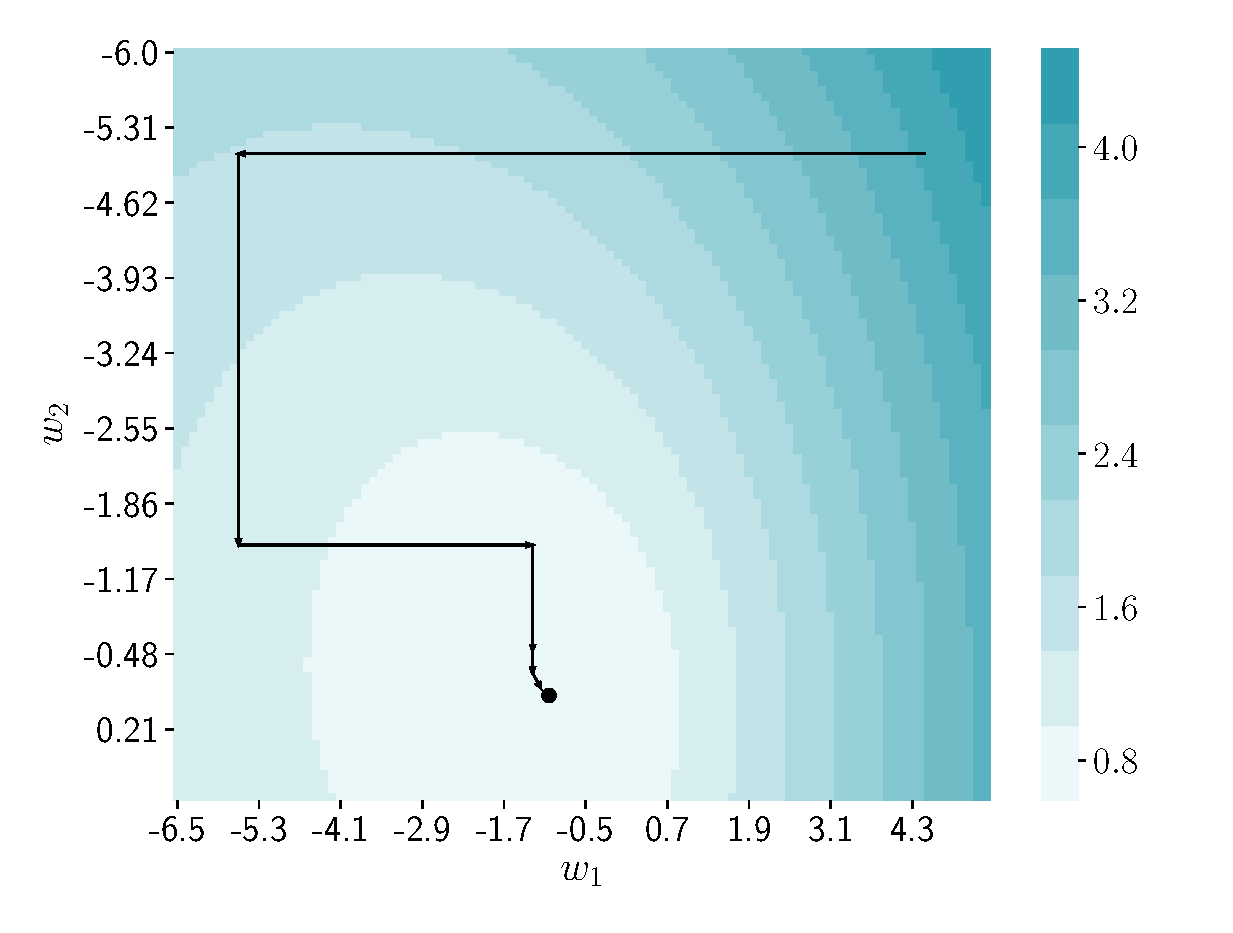
\includegraphics[width=0.6\linewidth]{figs/irls_qpfs_2d.eps}	 
		\caption{Optimization process for logistic regression with QPFS+Newton algorithm}
		\label{fig:irls_qpfs_2d}
	\end{figure}

	Figure~\ref{fig:active_params_wrt_iters} shows the sets of active parameters over iterations for Boston housing dataset and neural network with two 2 hidden neurons. The dark cells correspond to the active parameters that we optimize.

	\begin{figure}[!h]	
		\centering
		\includegraphics[width=\linewidth]{figs/active_params_wrt_iters.eps}	 
		\caption{Active parameters sets over optimization process}
		\label{fig:active_params_wrt_iters}
	\end{figure}
	
	In the considered examples the condition number~$\kappa (\bH)$ of the original Newton number in some iterations was extremely large. 
	The selection of the active parameters allowed to reduce the condition number significantly. 
	

	\section*{Conclusion}

  
  \bibliographystyle{unsrt}
  \bibliography{papers_qpfs.bib}
	\end{document}